% Drawn by scripts/revision3/fig_appendix_flows.py; the .pptx is the editable
% source and is released with the paper.
\begin{figure*}[t]
\centering
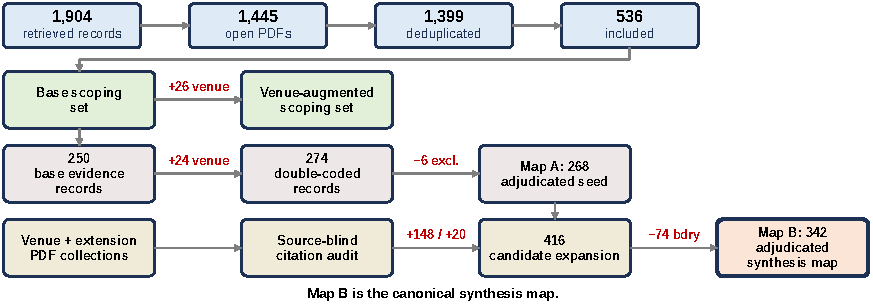
\includegraphics[width=\textwidth]{figures/generated/fig_corpus_lineage.pdf}%
\caption{Corpus lineage. Red deltas on the connectors are, in order, $+26$ and
$+24$ venue-linked additions, $-6$ exclusions, $+148$ new and $+20$ enriched
rows from the citation audit, and $-74$ boundary rows removed at adjudication.
The 416-row venue-expanded candidate map is second-coded and adjudicated into
Map~B (342 rows), the canonical synthesis evidence map. Map~A (268 rows) is the
double-coded adjudicated seed used for IAA and adjudication audit; the base and
venue-augmented scoping sets are used only for boundary checks, while a separate
300-paper source-blind citation audit over the venue and extension PDF
collections decides which papers enter the main text, case studies, or
appendix.}
\label{fig:corpus-flow}
\end{figure*}
